\chapter{Descripción del problema}

El objetivo del desarrollo de este proyecto es motivado debido a que el cuerpo policial utilizaba un esquema 
bastante anticuado para desemplear sus funciones y las convertía en tareas más complicadas, consiguiendo
una peor gestión del tiempo por parte del agente.\\

Por ejemplo, los registros de incidencias se iban apuntando manualmente y al final del turno se reunían para poner 
en común todos los datos en un documento que posteriormente se guardaba. Y al igual que en el ejemplo anterior, debían 
esperar a llegar a las dependencias para poder rellenar cualquier tipo de denuncia administrativa con los datos que habían
apuntado en un papel para no olvidarlos.\\

Para ello, he diseñado una aplicación web que se encarga de gestionar una gran cantidad de 
modelos de denuncia permitiendo que se rellenen de forma segura, a prueba de 
fallos y de una manera muy intuitiva para el usuario. Además de poder gestionar dichos documentos,
se ha creado un sistema de registro de incidencias completamente automatizado para que en 
ningún momento se pierda ningún dato y un gran número de funcionalidades más que se explicarán en 
posteriores puntos. El Ayuntamiento de Maracena será pionero en este ámbito, ya que han sido los 
primeros que han apostado por las nuevas tecnologías. Una gran apuesta, pero que traerá grandes
beneficios a la calidad del trabajo del cuerpo policial y a la seguridad de los ciudadanos. \\

A continuación, se enumeran de una manera general los apartados que se consiguen con 
este desarrollo:

\begin{enumerate}

    \item \textbf{Facilitar el trabajo a los policías locales de Maracena.}\\
    Debido a la inclusión de un sistema informatizado para la elaboración de 
    ficheros administrativos, gestión de incidentes y un sistema de croquis. Consiguiendo,
    por tanto, una mejora en la productividad de los agentes y un aumento de la seguridad
    global de los datos almacenados.
    
    \item \textbf{Inclusión del software libre en organismos del estado.}\\
    Dejando a un lado herramientas privativas sobre las que no tenemos un pleno control
    de los datos que están analizando y además fomentando el desarrollo libre. Porque 
    de esta manera cualquier persona puede sumarse al desarrollo y mejora de este software.

    \item \textbf{Elaboración de un entorno de pruebas real.}\\
    Se persigue la implementación de un entorno virtual lo más parecido posible a la 
    realidad para que el uso de la aplicación pueda ser probado antes del despliegue 
    final. 
   

   	
    \item \textbf{Probar los conocimientos adquiridos a lo largo del grado.}\\
    Creando un sistema completo en el que tendremos que tener en cuenta todos los 
    aspectos técnicos adquiridos en el transcurso de la carrera. Dada la embergadura del
    proyecto, es necesario disponer de una base muy consolidada de los conocimientos adquiridos
    previamente.
    
    
	% 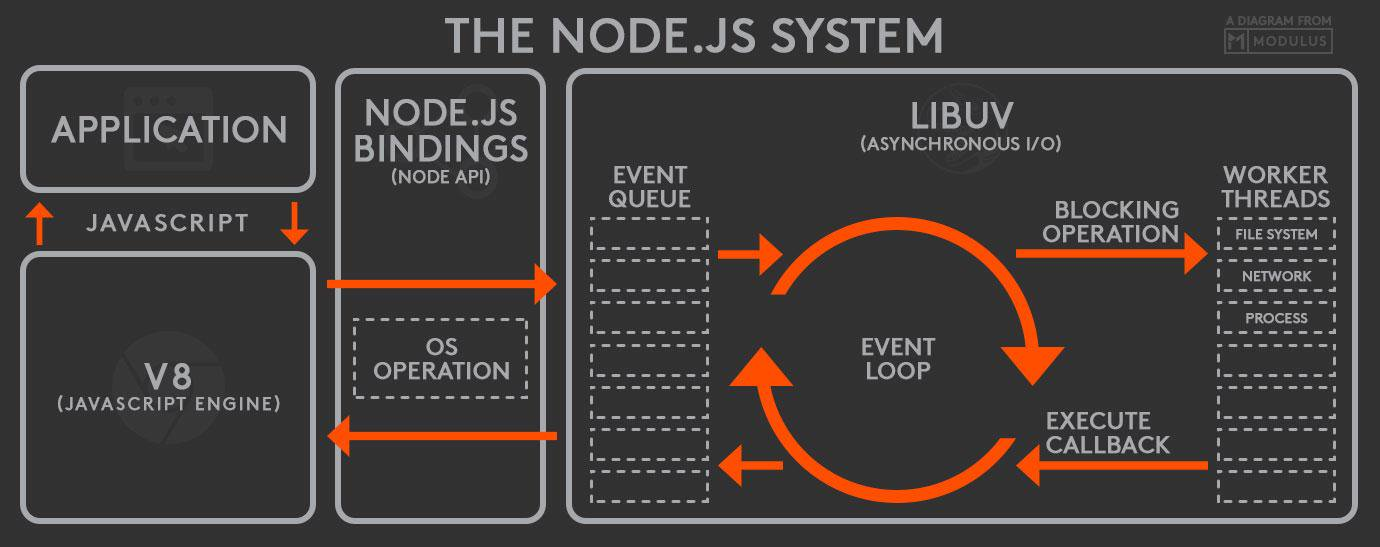
\includegraphics[scale=0.8]{imagenes/nodejs_system.jpg}
	
	\cite{gplv3}

    \item \textbf{Aprendizaje de tecnologías punteras en el sector.}\\
    Durante el desarollo del proyecto se ha buscado aprender y utilizar tecnologías en 
    auge que tienen un alto potencial. Esta decisión se toma en base  a la cantidad de gente
    y empresas que las utilizan, la comunidad tan amplia que tienen así como las contínuas
    mejoras que están recibiendo.  

\end{enumerate}
